\documentclass[1p]{elsarticle_modified}
%\bibliographystyle{elsarticle-num}

%\usepackage[colorlinks]{hyperref}
%\usepackage{abbrmath_seonhwa} %\Abb, \Ascr, \Acal ,\Abf, \Afrak
\usepackage{amsfonts}
\usepackage{amssymb}
\usepackage{amsmath}
\usepackage{amsthm}
\usepackage{scalefnt}
\usepackage{amsbsy}
\usepackage{kotex}
\usepackage{caption}
\usepackage{subfig}
\usepackage{color}
\usepackage{graphicx}
\usepackage{xcolor} %% white, black, red, green, blue, cyan, magenta, yellow
\usepackage{float}
\usepackage{setspace}
\usepackage{hyperref}

\usepackage{tikz}
\usetikzlibrary{arrows}

\usepackage{multirow}
\usepackage{array} % fixed length table
\usepackage{hhline}

%%%%%%%%%%%%%%%%%%%%%
\makeatletter
\renewcommand*\env@matrix[1][\arraystretch]{%
	\edef\arraystretch{#1}%
	\hskip -\arraycolsep
	\let\@ifnextchar\new@ifnextchar
	\array{*\c@MaxMatrixCols c}}
\makeatother %https://tex.stackexchange.com/questions/14071/how-can-i-increase-the-line-spacing-in-a-matrix
%%%%%%%%%%%%%%%

\usepackage[normalem]{ulem}

\newcommand{\msout}[1]{\ifmmode\text{\sout{\ensuremath{#1}}}\else\sout{#1}\fi}
%SOURCE: \msout is \stkout macro in https://tex.stackexchange.com/questions/20609/strikeout-in-math-mode

\newcommand{\cancel}[1]{
	\ifmmode
	{\color{red}\msout{#1}}
	\else
	{\color{red}\sout{#1}}
	\fi
}

\newcommand{\add}[1]{
	{\color{blue}\uwave{#1}}
}

\newcommand{\replace}[2]{
	\ifmmode
	{\color{red}\msout{#1}}{\color{blue}\uwave{#2}}
	\else
	{\color{red}\sout{#1}}{\color{blue}\uwave{#2}}
	\fi
}

\newcommand{\Sol}{\mathcal{S}} %segment
\newcommand{\D}{D} %diagram
\newcommand{\A}{\mathcal{A}} %arc


%%%%%%%%%%%%%%%%%%%%%%%%%%%%%5 test

\def\sl{\operatorname{\textup{SL}}(2,\Cbb)}
\def\psl{\operatorname{\textup{PSL}}(2,\Cbb)}
\def\quan{\mkern 1mu \triangleright \mkern 1mu}

\theoremstyle{definition}
\newtheorem{thm}{Theorem}[section]
\newtheorem{prop}[thm]{Proposition}
\newtheorem{lem}[thm]{Lemma}
\newtheorem{ques}[thm]{Question}
\newtheorem{cor}[thm]{Corollary}
\newtheorem{defn}[thm]{Definition}
\newtheorem{exam}[thm]{Example}
\newtheorem{rmk}[thm]{Remark}
\newtheorem{alg}[thm]{Algorithm}

\newcommand{\I}{\sqrt{-1}}
\begin{document}

%\begin{frontmatter}
%
%\title{Boundary parabolic representations of knots up to 8 crossings}
%
%%% Group authors per affiliation:
%\author{Yunhi Cho} 
%\address{Department of Mathematics, University of Seoul, Seoul, Korea}
%\ead{yhcho@uos.ac.kr}
%
%
%\author{Seonhwa Kim} %\fnref{s_kim}}
%\address{Center for Geometry and Physics, Institute for Basic Science, Pohang, 37673, Korea}
%\ead{ryeona17@ibs.re.kr}
%
%\author{Hyuk Kim}
%\address{Department of Mathematical Sciences, Seoul National University, Seoul 08826, Korea}
%\ead{hyukkim@snu.ac.kr}
%
%\author{Seokbeom Yoon}
%\address{Department of Mathematical Sciences, Seoul National University, Seoul, 08826,  Korea}
%\ead{sbyoon15@snu.ac.kr}
%
%\begin{abstract}
%We find all boundary parabolic representation of knots up to 8 crossings.
%
%\end{abstract}
%\begin{keyword}
%    \MSC[2010] 57M25 
%\end{keyword}
%
%\end{frontmatter}

%\linenumbers
%\tableofcontents
%
\newcommand\colored[1]{\textcolor{white}{\rule[-0.35ex]{0.8em}{1.4ex}}\kern-0.8em\color{red} #1}%
%\newcommand\colored[1]{\textcolor{white}{ #1}\kern-2.17ex	\textcolor{white}{ #1}\kern-1.81ex	\textcolor{white}{ #1}\kern-2.15ex\color{red}#1	}

{\Large $\underline{12n_{0659}~(K12n_{0659})}$}

\setlength{\tabcolsep}{10pt}
\renewcommand{\arraystretch}{1.6}
\vspace{1cm}\begin{tabular}{m{100pt}>{\centering\arraybackslash}m{274pt}}
\multirow{5}{120pt}{
	\centering
	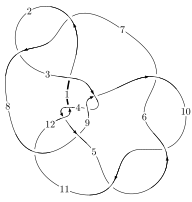
\includegraphics[width=112pt]{../../../GIT/diagram.site/Diagrams/png/2748_12n_0659.png}\\
\ \ \ A knot diagram\footnotemark}&
\allowdisplaybreaks
\textbf{Linearized knot diagam} \\
\cline{2-2}
 &
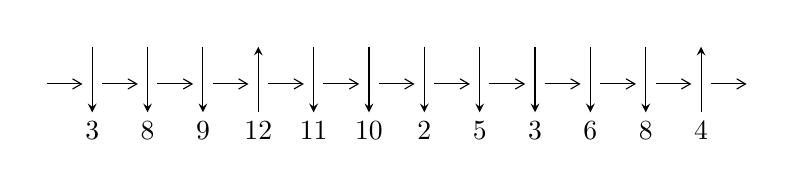
\begin{tikzpicture}[x=20pt, y=17pt]
	% nodes
	\node (C0) at (0, 0) {};
	\node (C1) at (1, 0) {};
	\node (C1U) at (1, +1) {};
	\node (C1D) at (1, -1) {3};

	\node (C2) at (2, 0) {};
	\node (C2U) at (2, +1) {};
	\node (C2D) at (2, -1) {8};

	\node (C3) at (3, 0) {};
	\node (C3U) at (3, +1) {};
	\node (C3D) at (3, -1) {9};

	\node (C4) at (4, 0) {};
	\node (C4U) at (4, +1) {};
	\node (C4D) at (4, -1) {12};

	\node (C5) at (5, 0) {};
	\node (C5U) at (5, +1) {};
	\node (C5D) at (5, -1) {11};

	\node (C6) at (6, 0) {};
	\node (C6U) at (6, +1) {};
	\node (C6D) at (6, -1) {10};

	\node (C7) at (7, 0) {};
	\node (C7U) at (7, +1) {};
	\node (C7D) at (7, -1) {2};

	\node (C8) at (8, 0) {};
	\node (C8U) at (8, +1) {};
	\node (C8D) at (8, -1) {5};

	\node (C9) at (9, 0) {};
	\node (C9U) at (9, +1) {};
	\node (C9D) at (9, -1) {3};

	\node (C10) at (10, 0) {};
	\node (C10U) at (10, +1) {};
	\node (C10D) at (10, -1) {6};

	\node (C11) at (11, 0) {};
	\node (C11U) at (11, +1) {};
	\node (C11D) at (11, -1) {8};

	\node (C12) at (12, 0) {};
	\node (C12U) at (12, +1) {};
	\node (C12D) at (12, -1) {4};
	\node (C13) at (13, 0) {};

	% arrows
	\draw[->,>={angle 60}]
	(C0) edge (C1) (C1) edge (C2) (C2) edge (C3) (C3) edge (C4) (C4) edge (C5) (C5) edge (C6) (C6) edge (C7) (C7) edge (C8) (C8) edge (C9) (C9) edge (C10) (C10) edge (C11) (C11) edge (C12) (C12) edge (C13) ;	\draw[->,>=stealth]
	(C1U) edge (C1D) (C2U) edge (C2D) (C3U) edge (C3D) (C4D) edge (C4U) (C5U) edge (C5D) (C6U) edge (C6D) (C7U) edge (C7D) (C8U) edge (C8D) (C9U) edge (C9D) (C10U) edge (C10D) (C11U) edge (C11D) (C12D) edge (C12U) ;
	\end{tikzpicture} \\
\hhline{~~} \\& 
\textbf{Solving Sequence} \\ \cline{2-2} 
 &
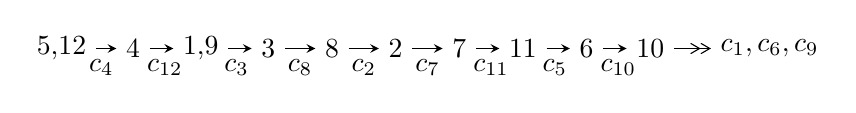
\begin{tikzpicture}[x=23pt, y=7pt]
	% node
	\node (A0) at (-1/8, 0) {5,12};
	\node (A1) at (1, 0) {4};
	\node (A2) at (33/16, 0) {1,9};
	\node (A3) at (25/8, 0) {3};
	\node (A4) at (33/8, 0) {8};
	\node (A5) at (41/8, 0) {2};
	\node (A6) at (49/8, 0) {7};
	\node (A7) at (57/8, 0) {11};
	\node (A8) at (65/8, 0) {6};
	\node (A9) at (73/8, 0) {10};
	\node (C1) at (1/2, -1) {$c_{4}$};
	\node (C2) at (3/2, -1) {$c_{12}$};
	\node (C3) at (21/8, -1) {$c_{3}$};
	\node (C4) at (29/8, -1) {$c_{8}$};
	\node (C5) at (37/8, -1) {$c_{2}$};
	\node (C6) at (45/8, -1) {$c_{7}$};
	\node (C7) at (53/8, -1) {$c_{11}$};
	\node (C8) at (61/8, -1) {$c_{5}$};
	\node (C9) at (69/8, -1) {$c_{10}$};
	\node (A10) at (11, 0) {$c_{1},c_{6},c_{9}$};

	% edge
	\draw[->,>=stealth]	
	(A0) edge (A1) (A1) edge (A2) (A2) edge (A3) (A3) edge (A4) (A4) edge (A5) (A5) edge (A6) (A6) edge (A7) (A7) edge (A8) (A8) edge (A9) ;
	\draw[->>,>={angle 60}]	
	(A9) edge (A10);
\end{tikzpicture} \\ 

\end{tabular} \\

\footnotetext{
The image of knot diagram is generated by the software ``\textbf{Draw programme}" developed by Andrew Bartholomew(\url{http://www.layer8.co.uk/maths/draw/index.htm\#Running-draw}), where we modified some parts for our purpose(\url{https://github.com/CATsTAILs/LinksPainter}).
}\phantom \\ \newline 
\centering \textbf{Ideals for irreducible components\footnotemark of $X_{\text{par}}$} 
 
\begin{align*}
I^u_{1}&=\langle 
-3.74446\times10^{123} u^{53}-1.80068\times10^{124} u^{52}+\cdots+2.83000\times10^{124} b-8.02256\times10^{125},\\
\phantom{I^u_{1}}&\phantom{= \langle  }1.03240\times10^{126} u^{53}+4.93019\times10^{126} u^{52}+\cdots+1.38670\times10^{126} a+2.28691\times10^{128},\\
\phantom{I^u_{1}}&\phantom{= \langle  }u^{54}+5 u^{53}+\cdots+528 u+49\rangle \\
I^u_{2}&=\langle 
2 u^{17}+16 u^{16}+\cdots+b+43,\;11 u^{17}-31 u^{16}+\cdots+a-24,\;u^{18}-2 u^{17}+\cdots-2 u+1\rangle \\
\\
\end{align*}
\raggedright * 2 irreducible components of $\dim_{\mathbb{C}}=0$, with total 72 representations.\\
\footnotetext{All coefficients of polynomials are rational numbers. But the coefficients are sometimes approximated in decimal forms when there is not enough margin.}
\newpage
\renewcommand{\arraystretch}{1}
\centering \section*{I. $I^u_{1}= \langle -3.74\times10^{123} u^{53}-1.80\times10^{124} u^{52}+\cdots+2.83\times10^{124} b-8.02\times10^{125},\;1.03\times10^{126} u^{53}+4.93\times10^{126} u^{52}+\cdots+1.39\times10^{126} a+2.29\times10^{128},\;u^{54}+5 u^{53}+\cdots+528 u+49 \rangle$}
\flushleft \textbf{(i) Arc colorings}\\
\begin{tabular}{m{7pt} m{180pt} m{7pt} m{180pt} }
\flushright $a_{5}=$&$\begin{pmatrix}1\\0\end{pmatrix}$ \\
\flushright $a_{12}=$&$\begin{pmatrix}0\\u\end{pmatrix}$ \\
\flushright $a_{4}=$&$\begin{pmatrix}1\\u^2\end{pmatrix}$ \\
\flushright $a_{1}=$&$\begin{pmatrix}u\\u^3+u\end{pmatrix}$ \\
\flushright $a_{9}=$&$\begin{pmatrix}-0.744500 u^{53}-3.55533 u^{52}+\cdots-1001.93 u-164.918\\0.132313 u^{53}+0.636282 u^{52}+\cdots+178.673 u+28.3483\end{pmatrix}$ \\
\flushright $a_{3}=$&$\begin{pmatrix}0.980752 u^{53}+4.70300 u^{52}+\cdots+1409.41 u+228.585\\-0.0620997 u^{53}-0.294145 u^{52}+\cdots-86.5558 u-14.5888\end{pmatrix}$ \\
\flushright $a_{8}=$&$\begin{pmatrix}-0.612187 u^{53}-2.91905 u^{52}+\cdots-823.256 u-136.569\\0.132313 u^{53}+0.636282 u^{52}+\cdots+178.673 u+28.3483\end{pmatrix}$ \\
\flushright $a_{2}=$&$\begin{pmatrix}2.27754 u^{53}+10.9226 u^{52}+\cdots+3266.86 u+527.076\\-0.155250 u^{53}-0.741079 u^{52}+\cdots-221.237 u-36.9171\end{pmatrix}$ \\
\flushright $a_{7}=$&$\begin{pmatrix}2.69305 u^{53}+12.8497 u^{52}+\cdots+3650.99 u+598.393\\-0.178103 u^{53}-0.850344 u^{52}+\cdots-239.834 u-38.4779\end{pmatrix}$ \\
\flushright $a_{11}=$&$\begin{pmatrix}-1.22947 u^{53}-5.89896 u^{52}+\cdots-1731.81 u-275.141\\0.129646 u^{53}+0.617545 u^{52}+\cdots+192.287 u+31.3383\end{pmatrix}$ \\
\flushright $a_{6}=$&$\begin{pmatrix}-1.12462 u^{53}-5.37150 u^{52}+\cdots-1476.98 u-234.162\\0.0650075 u^{53}+0.315357 u^{52}+\cdots+100.049 u+15.3130\end{pmatrix}$ \\
\flushright $a_{10}=$&$\begin{pmatrix}-1.86297 u^{53}-8.89331 u^{52}+\cdots-2509.47 u-410.424\\0.218460 u^{53}+1.04761 u^{52}+\cdots+297.149 u+47.1762\end{pmatrix}$\\&\end{tabular}
\flushleft \textbf{(ii) Obstruction class $= -1$}\\~\\
\flushleft \textbf{(iii) Cusp Shapes $= -0.164546 u^{53}-0.781563 u^{52}+\cdots-246.802 u-54.5462$}\\~\\
\newpage\renewcommand{\arraystretch}{1}
\flushleft \textbf{(iv) u-Polynomials at the component}\newline \\
\begin{tabular}{m{50pt}|m{274pt}}
Crossings & \hspace{64pt}u-Polynomials at each crossing \\
\hline $$\begin{aligned}c_{1}\end{aligned}$$&$\begin{aligned}
&u^{54}+57 u^{53}+\cdots+4309293 u+130321
\end{aligned}$\\
\hline $$\begin{aligned}c_{2},c_{7}\end{aligned}$$&$\begin{aligned}
&u^{54}+u^{53}+\cdots+1811 u-361
\end{aligned}$\\
\hline $$\begin{aligned}c_{3},c_{9}\end{aligned}$$&$\begin{aligned}
&u^{54}- u^{53}+\cdots-171 u-37
\end{aligned}$\\
\hline $$\begin{aligned}c_{4},c_{12}\end{aligned}$$&$\begin{aligned}
&u^{54}+5 u^{53}+\cdots+528 u+49
\end{aligned}$\\
\hline $$\begin{aligned}c_{5},c_{6},c_{10}\end{aligned}$$&$\begin{aligned}
&u^{54}+u^{53}+\cdots+146 u-143
\end{aligned}$\\
\hline $$\begin{aligned}c_{8}\end{aligned}$$&$\begin{aligned}
&u^{54}+3 u^{53}+\cdots-53 u-11
\end{aligned}$\\
\hline $$\begin{aligned}c_{11}\end{aligned}$$&$\begin{aligned}
&u^{54}-6 u^{52}+\cdots-2734 u+439
\end{aligned}$\\
\hline
\end{tabular}\\~\\
\newpage\renewcommand{\arraystretch}{1}
\flushleft \textbf{(v) Riley Polynomials at the component}\newline \\
\begin{tabular}{m{50pt}|m{274pt}}
Crossings & \hspace{64pt}Riley Polynomials at each crossing \\
\hline $$\begin{aligned}c_{1}\end{aligned}$$&$\begin{aligned}
&y^{54}-121 y^{53}+\cdots+1173617520891 y+16983563041
\end{aligned}$\\
\hline $$\begin{aligned}c_{2},c_{7}\end{aligned}$$&$\begin{aligned}
&y^{54}-57 y^{53}+\cdots-4309293 y+130321
\end{aligned}$\\
\hline $$\begin{aligned}c_{3},c_{9}\end{aligned}$$&$\begin{aligned}
&y^{54}-3 y^{53}+\cdots-82743 y+1369
\end{aligned}$\\
\hline $$\begin{aligned}c_{4},c_{12}\end{aligned}$$&$\begin{aligned}
&y^{54}+43 y^{53}+\cdots-40056 y+2401
\end{aligned}$\\
\hline $$\begin{aligned}c_{5},c_{6},c_{10}\end{aligned}$$&$\begin{aligned}
&y^{54}+43 y^{53}+\cdots+236656 y+20449
\end{aligned}$\\
\hline $$\begin{aligned}c_{8}\end{aligned}$$&$\begin{aligned}
&y^{54}+17 y^{53}+\cdots+1393 y+121
\end{aligned}$\\
\hline $$\begin{aligned}c_{11}\end{aligned}$$&$\begin{aligned}
&y^{54}-12 y^{53}+\cdots-2068032 y+192721
\end{aligned}$\\
\hline
\end{tabular}\\~\\
\newpage\flushleft \textbf{(vi) Complex Volumes and Cusp Shapes}
$$\begin{array}{c|c|c}  
\text{Solutions to }I^u_{1}& \I (\text{vol} + \sqrt{-1}CS) & \text{Cusp shape}\\
 \hline 
\begin{aligned}
u &= -0.234320 + 0.969892 I \\
a &= -0.148625 + 1.288510 I \\
b &= \phantom{-}0.475743 - 1.092990 I\end{aligned}
 & \phantom{-}3.14147 + 2.14385 I & -8.00000 - 2.27953 I \\ \hline\begin{aligned}
u &= -0.234320 - 0.969892 I \\
a &= -0.148625 - 1.288510 I \\
b &= \phantom{-}0.475743 + 1.092990 I\end{aligned}
 & \phantom{-}3.14147 - 2.14385 I & -8.00000 + 2.27953 I \\ \hline\begin{aligned}
u &= \phantom{-}0.027994 + 0.970519 I \\
a &= -0.553301 - 0.417496 I \\
b &= \phantom{-}0.36927 + 1.64804 I\end{aligned}
 & \phantom{-}3.04092 - 2.63323 I & -6.79514 + 3.39134 I \\ \hline\begin{aligned}
u &= \phantom{-}0.027994 - 0.970519 I \\
a &= -0.553301 + 0.417496 I \\
b &= \phantom{-}0.36927 - 1.64804 I\end{aligned}
 & \phantom{-}3.04092 + 2.63323 I & -6.79514 - 3.39134 I \\ \hline\begin{aligned}
u &= -0.782902 + 0.567024 I \\
a &= -0.515595 + 1.182860 I \\
b &= -0.368436 + 0.517578 I\end{aligned}
 & -2.46486 - 3.78662 I & -6.40927 + 1.45545 I \\ \hline\begin{aligned}
u &= -0.782902 - 0.567024 I \\
a &= -0.515595 - 1.182860 I \\
b &= -0.368436 - 0.517578 I\end{aligned}
 & -2.46486 + 3.78662 I & -6.40927 - 1.45545 I \\ \hline\begin{aligned}
u &= -0.362509 + 1.006200 I \\
a &= -1.74365 + 0.26534 I \\
b &= \phantom{-}1.03182 + 1.06263 I\end{aligned}
 & \phantom{-}2.07901 - 4.91557 I & -8.00000 + 0. I\phantom{ +0.000000I} \\ \hline\begin{aligned}
u &= -0.362509 - 1.006200 I \\
a &= -1.74365 - 0.26534 I \\
b &= \phantom{-}1.03182 - 1.06263 I\end{aligned}
 & \phantom{-}2.07901 + 4.91557 I & -8.00000 + 0. I\phantom{ +0.000000I} \\ \hline\begin{aligned}
u &= \phantom{-}0.562881 + 1.010060 I \\
a &= \phantom{-}1.70829 + 0.19125 I \\
b &= -1.08761 + 0.91934 I\end{aligned}
 & \phantom{-}0.36171 + 5.69112 I & \phantom{-0.000000 } 0 \\ \hline\begin{aligned}
u &= \phantom{-}0.562881 - 1.010060 I \\
a &= \phantom{-}1.70829 - 0.19125 I \\
b &= -1.08761 - 0.91934 I\end{aligned}
 & \phantom{-}0.36171 - 5.69112 I & \phantom{-0.000000 } 0\\
 \hline 
 \end{array}$$\newpage$$\begin{array}{c|c|c}  
\text{Solutions to }I^u_{1}& \I (\text{vol} + \sqrt{-1}CS) & \text{Cusp shape}\\
 \hline 
\begin{aligned}
u &= -0.311601 + 1.189300 I \\
a &= \phantom{-}1.261750 - 0.239301 I \\
b &= -0.846614 - 0.808655 I\end{aligned}
 & -3.40881 - 2.20781 I & \phantom{-0.000000 } 0 \\ \hline\begin{aligned}
u &= -0.311601 - 1.189300 I \\
a &= \phantom{-}1.261750 + 0.239301 I \\
b &= -0.846614 + 0.808655 I\end{aligned}
 & -3.40881 + 2.20781 I & \phantom{-0.000000 } 0 \\ \hline\begin{aligned}
u &= \phantom{-}0.475047 + 0.535369 I \\
a &= \phantom{-}0.075261 + 0.763788 I \\
b &= -0.550857 - 1.221260 I\end{aligned}
 & \phantom{-}2.01849 - 1.23122 I & -3.26105 - 1.16198 I \\ \hline\begin{aligned}
u &= \phantom{-}0.475047 - 0.535369 I \\
a &= \phantom{-}0.075261 - 0.763788 I \\
b &= -0.550857 + 1.221260 I\end{aligned}
 & \phantom{-}2.01849 + 1.23122 I & -3.26105 + 1.16198 I \\ \hline\begin{aligned}
u &= \phantom{-}0.465598 + 1.208790 I \\
a &= -1.173780 + 0.049718 I \\
b &= \phantom{-}0.795766 - 0.488765 I\end{aligned}
 & -1.16225 + 2.99382 I & \phantom{-0.000000 } 0 \\ \hline\begin{aligned}
u &= \phantom{-}0.465598 - 1.208790 I \\
a &= -1.173780 - 0.049718 I \\
b &= \phantom{-}0.795766 + 0.488765 I\end{aligned}
 & -1.16225 - 2.99382 I & \phantom{-0.000000 } 0 \\ \hline\begin{aligned}
u &= -0.665299 + 1.133700 I \\
a &= \phantom{-}0.975711 - 0.647626 I \\
b &= -0.441264 - 0.844294 I\end{aligned}
 & -4.11326 - 2.05845 I & \phantom{-0.000000 } 0 \\ \hline\begin{aligned}
u &= -0.665299 - 1.133700 I \\
a &= \phantom{-}0.975711 + 0.647626 I \\
b &= -0.441264 + 0.844294 I\end{aligned}
 & -4.11326 + 2.05845 I & \phantom{-0.000000 } 0 \\ \hline\begin{aligned}
u &= \phantom{-}0.039718 + 1.317490 I \\
a &= -1.060890 - 0.018811 I \\
b &= \phantom{-}0.932021 + 0.518191 I\end{aligned}
 & -2.35880 + 2.03182 I & \phantom{-0.000000 } 0 \\ \hline\begin{aligned}
u &= \phantom{-}0.039718 - 1.317490 I \\
a &= -1.060890 + 0.018811 I \\
b &= \phantom{-}0.932021 - 0.518191 I\end{aligned}
 & -2.35880 - 2.03182 I & \phantom{-0.000000 } 0\\
 \hline 
 \end{array}$$\newpage$$\begin{array}{c|c|c}  
\text{Solutions to }I^u_{1}& \I (\text{vol} + \sqrt{-1}CS) & \text{Cusp shape}\\
 \hline 
\begin{aligned}
u &= \phantom{-}0.352052 + 0.575861 I \\
a &= \phantom{-}0.49680 - 1.33952 I \\
b &= \phantom{-}0.143466 - 1.197570 I\end{aligned}
 & \phantom{-}8.88135 + 1.75033 I & -0.23249 - 5.30216 I \\ \hline\begin{aligned}
u &= \phantom{-}0.352052 - 0.575861 I \\
a &= \phantom{-}0.49680 + 1.33952 I \\
b &= \phantom{-}0.143466 + 1.197570 I\end{aligned}
 & \phantom{-}8.88135 - 1.75033 I & -0.23249 + 5.30216 I \\ \hline\begin{aligned}
u &= \phantom{-}0.103091 + 1.329410 I \\
a &= \phantom{-}1.221790 + 0.330306 I \\
b &= -0.717176 + 1.156320 I\end{aligned}
 & -6.43910 + 4.65775 I & \phantom{-0.000000 } 0 \\ \hline\begin{aligned}
u &= \phantom{-}0.103091 - 1.329410 I \\
a &= \phantom{-}1.221790 - 0.330306 I \\
b &= -0.717176 - 1.156320 I\end{aligned}
 & -6.43910 - 4.65775 I & \phantom{-0.000000 } 0 \\ \hline\begin{aligned}
u &= \phantom{-}0.655732 + 0.001796 I \\
a &= -0.426767 - 0.217995 I \\
b &= -0.216342 + 0.945304 I\end{aligned}
 & \phantom{-}2.33536 + 1.33301 I & -3.31811 - 4.81791 I \\ \hline\begin{aligned}
u &= \phantom{-}0.655732 - 0.001796 I \\
a &= -0.426767 + 0.217995 I \\
b &= -0.216342 - 0.945304 I\end{aligned}
 & \phantom{-}2.33536 - 1.33301 I & -3.31811 + 4.81791 I \\ \hline\begin{aligned}
u &= -0.099058 + 1.403950 I \\
a &= -1.200600 + 0.034439 I \\
b &= \phantom{-}1.00529 - 0.99657 I\end{aligned}
 & -11.55370 - 1.21518 I & \phantom{-0.000000 } 0 \\ \hline\begin{aligned}
u &= -0.099058 - 1.403950 I \\
a &= -1.200600 - 0.034439 I \\
b &= \phantom{-}1.00529 + 0.99657 I\end{aligned}
 & -11.55370 + 1.21518 I & \phantom{-0.000000 } 0 \\ \hline\begin{aligned}
u &= \phantom{-}1.383890 + 0.257220 I \\
a &= \phantom{-}0.042622 + 0.310020 I \\
b &= \phantom{-}0.327830 + 0.748998 I\end{aligned}
 & \phantom{-}4.07354 - 1.34058 I & \phantom{-0.000000 } 0 \\ \hline\begin{aligned}
u &= \phantom{-}1.383890 - 0.257220 I \\
a &= \phantom{-}0.042622 - 0.310020 I \\
b &= \phantom{-}0.327830 - 0.748998 I\end{aligned}
 & \phantom{-}4.07354 + 1.34058 I & \phantom{-0.000000 } 0\\
 \hline 
 \end{array}$$\newpage$$\begin{array}{c|c|c}  
\text{Solutions to }I^u_{1}& \I (\text{vol} + \sqrt{-1}CS) & \text{Cusp shape}\\
 \hline 
\begin{aligned}
u &= -0.304294 + 0.499465 I \\
a &= \phantom{-}1.02836 + 1.02465 I \\
b &= \phantom{-}0.511575 - 0.716466 I\end{aligned}
 & \phantom{-}3.32556 + 1.82215 I & -7.68501 - 4.30894 I \\ \hline\begin{aligned}
u &= -0.304294 - 0.499465 I \\
a &= \phantom{-}1.02836 - 1.02465 I \\
b &= \phantom{-}0.511575 + 0.716466 I\end{aligned}
 & \phantom{-}3.32556 - 1.82215 I & -7.68501 + 4.30894 I \\ \hline\begin{aligned}
u &= -0.29988 + 1.38353 I \\
a &= \phantom{-}1.167220 - 0.318667 I \\
b &= -1.25222 + 0.74442 I\end{aligned}
 & -8.06461 - 7.14617 I & \phantom{-0.000000 } 0 \\ \hline\begin{aligned}
u &= -0.29988 - 1.38353 I \\
a &= \phantom{-}1.167220 + 0.318667 I \\
b &= -1.25222 - 0.74442 I\end{aligned}
 & -8.06461 + 7.14617 I & \phantom{-0.000000 } 0 \\ \hline\begin{aligned}
u &= -1.44175 + 0.12669 I \\
a &= \phantom{-}0.163034 - 0.101692 I \\
b &= -0.564264 - 0.875736 I\end{aligned}
 & -1.51180 - 7.69812 I & \phantom{-0.000000 } 0 \\ \hline\begin{aligned}
u &= -1.44175 - 0.12669 I \\
a &= \phantom{-}0.163034 + 0.101692 I \\
b &= -0.564264 + 0.875736 I\end{aligned}
 & -1.51180 + 7.69812 I & \phantom{-0.000000 } 0 \\ \hline\begin{aligned}
u &= \phantom{-}0.41538 + 1.39497 I \\
a &= \phantom{-}0.473978 - 0.650086 I \\
b &= \phantom{-}0.037314 + 0.438841 I\end{aligned}
 & \phantom{-}5.88808 + 0.92042 I & \phantom{-0.000000 } 0 \\ \hline\begin{aligned}
u &= \phantom{-}0.41538 - 1.39497 I \\
a &= \phantom{-}0.473978 + 0.650086 I \\
b &= \phantom{-}0.037314 - 0.438841 I\end{aligned}
 & \phantom{-}5.88808 - 0.92042 I & \phantom{-0.000000 } 0 \\ \hline\begin{aligned}
u &= \phantom{-}0.25489 + 1.47796 I \\
a &= \phantom{-}0.911154 - 0.269340 I \\
b &= -0.801265 + 0.938714 I\end{aligned}
 & -3.02616 + 3.86573 I & \phantom{-0.000000 } 0 \\ \hline\begin{aligned}
u &= \phantom{-}0.25489 - 1.47796 I \\
a &= \phantom{-}0.911154 + 0.269340 I \\
b &= -0.801265 - 0.938714 I\end{aligned}
 & -3.02616 - 3.86573 I & \phantom{-0.000000 } 0\\
 \hline 
 \end{array}$$\newpage$$\begin{array}{c|c|c}  
\text{Solutions to }I^u_{1}& \I (\text{vol} + \sqrt{-1}CS) & \text{Cusp shape}\\
 \hline 
\begin{aligned}
u &= \phantom{-}0.56773 + 1.48140 I \\
a &= -1.040690 + 0.016279 I \\
b &= \phantom{-}0.752725 - 1.177120 I\end{aligned}
 & -0.36984 + 8.31182 I & \phantom{-0.000000 } 0 \\ \hline\begin{aligned}
u &= \phantom{-}0.56773 - 1.48140 I \\
a &= -1.040690 - 0.016279 I \\
b &= \phantom{-}0.752725 + 1.177120 I\end{aligned}
 & -0.36984 - 8.31182 I & \phantom{-0.000000 } 0 \\ \hline\begin{aligned}
u &= -0.63065 + 1.50296 I \\
a &= \phantom{-}1.250760 + 0.035031 I \\
b &= -0.91992 - 1.19790 I\end{aligned}
 & -6.5506 - 14.8339 I & \phantom{-0.000000 } 0 \\ \hline\begin{aligned}
u &= -0.63065 - 1.50296 I \\
a &= \phantom{-}1.250760 - 0.035031 I \\
b &= -0.91992 + 1.19790 I\end{aligned}
 & -6.5506 + 14.8339 I & \phantom{-0.000000 } 0 \\ \hline\begin{aligned}
u &= -0.149852 + 0.300455 I \\
a &= -1.23317 + 5.69132 I \\
b &= -0.541979 - 0.188288 I\end{aligned}
 & -2.60231 - 4.18203 I & -11.45087 - 0.72915 I \\ \hline\begin{aligned}
u &= -0.149852 - 0.300455 I \\
a &= -1.23317 - 5.69132 I \\
b &= -0.541979 + 0.188288 I\end{aligned}
 & -2.60231 + 4.18203 I & -11.45087 + 0.72915 I \\ \hline\begin{aligned}
u &= -0.51673 + 1.64071 I \\
a &= -1.063790 - 0.161215 I \\
b &= \phantom{-}0.980622 + 0.969393 I\end{aligned}
 & -11.5956 - 8.4499 I & \phantom{-0.000000 } 0 \\ \hline\begin{aligned}
u &= -0.51673 - 1.64071 I \\
a &= -1.063790 + 0.161215 I \\
b &= \phantom{-}0.980622 - 0.969393 I\end{aligned}
 & -11.5956 + 8.4499 I & \phantom{-0.000000 } 0 \\ \hline\begin{aligned}
u &= -1.48162 + 0.91100 I \\
a &= -0.133736 - 0.101440 I \\
b &= \phantom{-}0.190419 + 0.615231 I\end{aligned}
 & -4.30577 - 1.29948 I & \phantom{-0.000000 } 0 \\ \hline\begin{aligned}
u &= -1.48162 - 0.91100 I \\
a &= -0.133736 + 0.101440 I \\
b &= \phantom{-}0.190419 - 0.615231 I\end{aligned}
 & -4.30577 + 1.29948 I & \phantom{-0.000000 } 0\\
 \hline 
 \end{array}$$\newpage$$\begin{array}{c|c|c}  
\text{Solutions to }I^u_{1}& \I (\text{vol} + \sqrt{-1}CS) & \text{Cusp shape}\\
 \hline 
\begin{aligned}
u &= -0.30454 + 1.73276 I \\
a &= \phantom{-}0.825545 + 0.324392 I \\
b &= -0.878673 - 0.649779 I\end{aligned}
 & -8.04995 - 1.38990 I & \phantom{-0.000000 } 0 \\ \hline\begin{aligned}
u &= -0.30454 - 1.73276 I \\
a &= \phantom{-}0.825545 - 0.324392 I \\
b &= -0.878673 + 0.649779 I\end{aligned}
 & -8.04995 + 1.38990 I & \phantom{-0.000000 } 0 \\ \hline\begin{aligned}
u &= -0.221783\phantom{ +0.000000I} \\
a &= -1.37508\phantom{ +0.000000I} \\
b &= -0.409309\phantom{ +0.000000I}\end{aligned}
 & -0.627945\phantom{ +0.000000I} & -15.7990\phantom{ +0.000000I} \\ \hline\begin{aligned}
u &= -0.216213\phantom{ +0.000000I} \\
a &= -7.73007\phantom{ +0.000000I} \\
b &= \phantom{-}0.674840\phantom{ +0.000000I}\end{aligned}
 & -6.62446\phantom{ +0.000000I} & -17.2110\phantom{ +0.000000I}\\
 \hline 
 \end{array}$$\newpage\newpage\renewcommand{\arraystretch}{1}
\centering \section*{II. $I^u_{2}= \langle 2 u^{17}+16 u^{16}+\cdots+b+43,\;11 u^{17}-31 u^{16}+\cdots+a-24,\;u^{18}-2 u^{17}+\cdots-2 u+1 \rangle$}
\flushleft \textbf{(i) Arc colorings}\\
\begin{tabular}{m{7pt} m{180pt} m{7pt} m{180pt} }
\flushright $a_{5}=$&$\begin{pmatrix}1\\0\end{pmatrix}$ \\
\flushright $a_{12}=$&$\begin{pmatrix}0\\u\end{pmatrix}$ \\
\flushright $a_{4}=$&$\begin{pmatrix}1\\u^2\end{pmatrix}$ \\
\flushright $a_{1}=$&$\begin{pmatrix}u\\u^3+u\end{pmatrix}$ \\
\flushright $a_{9}=$&$\begin{pmatrix}-11 u^{17}+31 u^{16}+\cdots-48 u+24\\-2 u^{17}-16 u^{16}+\cdots+60 u-43\end{pmatrix}$ \\
\flushright $a_{3}=$&$\begin{pmatrix}-3 u^{17}+10 u^{16}+\cdots+32 u^2-9 u\\u^{16}-2 u^{15}+\cdots-2 u+2\end{pmatrix}$ \\
\flushright $a_{8}=$&$\begin{pmatrix}-13 u^{17}+15 u^{16}+\cdots+12 u-19\\-2 u^{17}-16 u^{16}+\cdots+60 u-43\end{pmatrix}$ \\
\flushright $a_{2}=$&$\begin{pmatrix}-7 u^{17}+19 u^{16}+\cdots-34 u+6\\u^{17}- u^{16}+\cdots-5 u^2+7 u\end{pmatrix}$ \\
\flushright $a_{7}=$&$\begin{pmatrix}11 u^{17}-8 u^{16}+\cdots-10 u+19\\-2 u^{17}+8 u^{16}+\cdots-12 u+4\end{pmatrix}$ \\
\flushright $a_{11}=$&$\begin{pmatrix}-12 u^{17}+17 u^{16}+\cdots+4 u-11\\u^{16}+4 u^{14}+\cdots+2 u+5\end{pmatrix}$ \\
\flushright $a_{6}=$&$\begin{pmatrix}19 u^{17}-56 u^{16}+\cdots+94 u-30\\19 u^{17}-41 u^{16}+\cdots+58 u-13\end{pmatrix}$ \\
\flushright $a_{10}=$&$\begin{pmatrix}35 u^{17}-51 u^{16}+\cdots+16 u+31\\9 u^{17}-10 u^{16}+\cdots-7 u+10\end{pmatrix}$\\&\end{tabular}
\flushleft \textbf{(ii) Obstruction class $= 1$}\\~\\
\flushleft \textbf{(iii) Cusp Shapes $= -116 u^{17}+218 u^{16}-732 u^{15}+1098 u^{14}-2099 u^{13}+3132 u^{12}-4657 u^{11}+6171 u^{10}-6988 u^9+6776 u^8-6308 u^7+4541 u^6-4126 u^5+2176 u^4-1742 u^3+599 u^2-297 u+39$}\\~\\
\newpage\renewcommand{\arraystretch}{1}
\flushleft \textbf{(iv) u-Polynomials at the component}\newline \\
\begin{tabular}{m{50pt}|m{274pt}}
Crossings & \hspace{64pt}u-Polynomials at each crossing \\
\hline $$\begin{aligned}c_{1}\end{aligned}$$&$\begin{aligned}
&u^{18}-14 u^{17}+\cdots-11 u+1
\end{aligned}$\\
\hline $$\begin{aligned}c_{2}\end{aligned}$$&$\begin{aligned}
&u^{18}-7 u^{16}+\cdots+u+1
\end{aligned}$\\
\hline $$\begin{aligned}c_{3}\end{aligned}$$&$\begin{aligned}
&u^{18}+6 u^{16}+\cdots- u+1
\end{aligned}$\\
\hline $$\begin{aligned}c_{4}\end{aligned}$$&$\begin{aligned}
&u^{18}-2 u^{17}+\cdots-2 u+1
\end{aligned}$\\
\hline $$\begin{aligned}c_{5},c_{6}\end{aligned}$$&$\begin{aligned}
&u^{18}+11 u^{16}+\cdots-4 u+1
\end{aligned}$\\
\hline $$\begin{aligned}c_{7}\end{aligned}$$&$\begin{aligned}
&u^{18}-7 u^{16}+\cdots- u+1
\end{aligned}$\\
\hline $$\begin{aligned}c_{8}\end{aligned}$$&$\begin{aligned}
&u^{18}-2 u^{17}+\cdots-3 u+1
\end{aligned}$\\
\hline $$\begin{aligned}c_{9}\end{aligned}$$&$\begin{aligned}
&u^{18}+6 u^{16}+\cdots+u+1
\end{aligned}$\\
\hline $$\begin{aligned}c_{10}\end{aligned}$$&$\begin{aligned}
&u^{18}+11 u^{16}+\cdots+4 u+1
\end{aligned}$\\
\hline $$\begin{aligned}c_{11}\end{aligned}$$&$\begin{aligned}
&u^{18}- u^{17}+\cdots-11 u^2+1
\end{aligned}$\\
\hline $$\begin{aligned}c_{12}\end{aligned}$$&$\begin{aligned}
&u^{18}+2 u^{17}+\cdots+2 u+1
\end{aligned}$\\
\hline
\end{tabular}\\~\\
\newpage\renewcommand{\arraystretch}{1}
\flushleft \textbf{(v) Riley Polynomials at the component}\newline \\
\begin{tabular}{m{50pt}|m{274pt}}
Crossings & \hspace{64pt}Riley Polynomials at each crossing \\
\hline $$\begin{aligned}c_{1}\end{aligned}$$&$\begin{aligned}
&y^{18}-22 y^{17}+\cdots+y+1
\end{aligned}$\\
\hline $$\begin{aligned}c_{2},c_{7}\end{aligned}$$&$\begin{aligned}
&y^{18}-14 y^{17}+\cdots-11 y+1
\end{aligned}$\\
\hline $$\begin{aligned}c_{3},c_{9}\end{aligned}$$&$\begin{aligned}
&y^{18}+12 y^{17}+\cdots+11 y+1
\end{aligned}$\\
\hline $$\begin{aligned}c_{4},c_{12}\end{aligned}$$&$\begin{aligned}
&y^{18}+10 y^{17}+\cdots+14 y+1
\end{aligned}$\\
\hline $$\begin{aligned}c_{5},c_{6},c_{10}\end{aligned}$$&$\begin{aligned}
&y^{18}+22 y^{17}+\cdots+14 y+1
\end{aligned}$\\
\hline $$\begin{aligned}c_{8}\end{aligned}$$&$\begin{aligned}
&y^{18}+12 y^{17}+\cdots+11 y+1
\end{aligned}$\\
\hline $$\begin{aligned}c_{11}\end{aligned}$$&$\begin{aligned}
&y^{18}- y^{17}+\cdots-22 y+1
\end{aligned}$\\
\hline
\end{tabular}\\~\\
\newpage\flushleft \textbf{(vi) Complex Volumes and Cusp Shapes}
$$\begin{array}{c|c|c}  
\text{Solutions to }I^u_{2}& \I (\text{vol} + \sqrt{-1}CS) & \text{Cusp shape}\\
 \hline 
\begin{aligned}
u &= \phantom{-}0.433983 + 1.043760 I \\
a &= \phantom{-}1.76917 + 0.06570 I \\
b &= -1.10704 + 1.10280 I\end{aligned}
 & \phantom{-}2.38044 + 5.58075 I & -3.29349 - 9.18069 I \\ \hline\begin{aligned}
u &= \phantom{-}0.433983 - 1.043760 I \\
a &= \phantom{-}1.76917 - 0.06570 I \\
b &= -1.10704 - 1.10280 I\end{aligned}
 & \phantom{-}2.38044 - 5.58075 I & -3.29349 + 9.18069 I \\ \hline\begin{aligned}
u &= \phantom{-}1.109000 + 0.375523 I \\
a &= -0.336175 - 0.040796 I \\
b &= -0.330973 - 0.824788 I\end{aligned}
 & \phantom{-}4.68841 - 1.16029 I & \phantom{-}1.77241 + 1.34126 I \\ \hline\begin{aligned}
u &= \phantom{-}1.109000 - 0.375523 I \\
a &= -0.336175 + 0.040796 I \\
b &= -0.330973 + 0.824788 I\end{aligned}
 & \phantom{-}4.68841 + 1.16029 I & \phantom{-}1.77241 - 1.34126 I \\ \hline\begin{aligned}
u &= -0.527284 + 0.639053 I \\
a &= -1.03264 + 2.28395 I \\
b &= \phantom{-}0.542663 + 0.578885 I\end{aligned}
 & -2.36972 - 4.87568 I & -7.53244 + 9.08177 I \\ \hline\begin{aligned}
u &= -0.527284 - 0.639053 I \\
a &= -1.03264 - 2.28395 I \\
b &= \phantom{-}0.542663 - 0.578885 I\end{aligned}
 & -2.36972 + 4.87568 I & -7.53244 - 9.08177 I \\ \hline\begin{aligned}
u &= \phantom{-}0.030219 + 0.770891 I \\
a &= \phantom{-}0.89608 - 1.10632 I \\
b &= -0.275066 - 1.229750 I\end{aligned}
 & \phantom{-}8.30714 - 1.03793 I & -7.10521 - 1.06063 I \\ \hline\begin{aligned}
u &= \phantom{-}0.030219 - 0.770891 I \\
a &= \phantom{-}0.89608 + 1.10632 I \\
b &= -0.275066 + 1.229750 I\end{aligned}
 & \phantom{-}8.30714 + 1.03793 I & -7.10521 + 1.06063 I \\ \hline\begin{aligned}
u &= \phantom{-}0.441547 + 1.178770 I \\
a &= -1.208310 + 0.169945 I \\
b &= \phantom{-}0.835779 - 0.722556 I\end{aligned}
 & -1.27644 + 3.83272 I & -8.04046 - 6.78992 I \\ \hline\begin{aligned}
u &= \phantom{-}0.441547 - 1.178770 I \\
a &= -1.208310 - 0.169945 I \\
b &= \phantom{-}0.835779 + 0.722556 I\end{aligned}
 & -1.27644 - 3.83272 I & -8.04046 + 6.78992 I\\
 \hline 
 \end{array}$$\newpage$$\begin{array}{c|c|c}  
\text{Solutions to }I^u_{2}& \I (\text{vol} + \sqrt{-1}CS) & \text{Cusp shape}\\
 \hline 
\begin{aligned}
u &= \phantom{-}0.090717 + 0.687766 I \\
a &= -0.811399 - 0.398978 I \\
b &= \phantom{-}0.37619 + 1.36678 I\end{aligned}
 & \phantom{-}1.34686 - 1.58107 I & -12.80363 + 3.25466 I \\ \hline\begin{aligned}
u &= \phantom{-}0.090717 - 0.687766 I \\
a &= -0.811399 + 0.398978 I \\
b &= \phantom{-}0.37619 - 1.36678 I\end{aligned}
 & \phantom{-}1.34686 + 1.58107 I & -12.80363 - 3.25466 I \\ \hline\begin{aligned}
u &= \phantom{-}0.186640 + 0.604958 I \\
a &= \phantom{-}0.03137 + 1.98200 I \\
b &= -0.47824 - 1.53175 I\end{aligned}
 & \phantom{-}4.32414 - 2.28815 I & \phantom{-}0.92523 + 2.22693 I \\ \hline\begin{aligned}
u &= \phantom{-}0.186640 - 0.604958 I \\
a &= \phantom{-}0.03137 - 1.98200 I \\
b &= -0.47824 + 1.53175 I\end{aligned}
 & \phantom{-}4.32414 + 2.28815 I & \phantom{-}0.92523 - 2.22693 I \\ \hline\begin{aligned}
u &= -0.93428 + 1.11326 I \\
a &= \phantom{-}0.409560 - 0.526106 I \\
b &= -0.240017 - 0.368514 I\end{aligned}
 & -5.08793 - 1.14055 I & -13.57284 + 0.84904 I \\ \hline\begin{aligned}
u &= -0.93428 - 1.11326 I \\
a &= \phantom{-}0.409560 + 0.526106 I \\
b &= -0.240017 + 0.368514 I\end{aligned}
 & -5.08793 + 1.14055 I & -13.57284 - 0.84904 I \\ \hline\begin{aligned}
u &= \phantom{-}0.16946 + 1.46145 I \\
a &= \phantom{-}0.282355 - 0.799726 I \\
b &= -0.323299 + 0.565718 I\end{aligned}
 & \phantom{-}5.78138 + 1.58656 I & -4.84957 - 7.40440 I \\ \hline\begin{aligned}
u &= \phantom{-}0.16946 - 1.46145 I \\
a &= \phantom{-}0.282355 + 0.799726 I \\
b &= -0.323299 - 0.565718 I\end{aligned}
 & \phantom{-}5.78138 - 1.58656 I & -4.84957 + 7.40440 I\\
 \hline 
 \end{array}$$\newpage
\newpage\renewcommand{\arraystretch}{1}
\centering \section*{ III. u-Polynomials}
\begin{tabular}{m{50pt}|m{274pt}}
Crossings & \hspace{64pt}u-Polynomials at each crossing \\
\hline $$\begin{aligned}c_{1}\end{aligned}$$&$\begin{aligned}
&(u^{18}-14 u^{17}+\cdots-11 u+1)\\
&\cdot(u^{54}+57 u^{53}+\cdots+4309293 u+130321)
\end{aligned}$\\
\hline $$\begin{aligned}c_{2}\end{aligned}$$&$\begin{aligned}
&(u^{18}-7 u^{16}+\cdots+u+1)(u^{54}+u^{53}+\cdots+1811 u-361)
\end{aligned}$\\
\hline $$\begin{aligned}c_{3}\end{aligned}$$&$\begin{aligned}
&(u^{18}+6 u^{16}+\cdots- u+1)(u^{54}- u^{53}+\cdots-171 u-37)
\end{aligned}$\\
\hline $$\begin{aligned}c_{4}\end{aligned}$$&$\begin{aligned}
&(u^{18}-2 u^{17}+\cdots-2 u+1)(u^{54}+5 u^{53}+\cdots+528 u+49)
\end{aligned}$\\
\hline $$\begin{aligned}c_{5},c_{6}\end{aligned}$$&$\begin{aligned}
&(u^{18}+11 u^{16}+\cdots-4 u+1)(u^{54}+u^{53}+\cdots+146 u-143)
\end{aligned}$\\
\hline $$\begin{aligned}c_{7}\end{aligned}$$&$\begin{aligned}
&(u^{18}-7 u^{16}+\cdots- u+1)(u^{54}+u^{53}+\cdots+1811 u-361)
\end{aligned}$\\
\hline $$\begin{aligned}c_{8}\end{aligned}$$&$\begin{aligned}
&(u^{18}-2 u^{17}+\cdots-3 u+1)(u^{54}+3 u^{53}+\cdots-53 u-11)
\end{aligned}$\\
\hline $$\begin{aligned}c_{9}\end{aligned}$$&$\begin{aligned}
&(u^{18}+6 u^{16}+\cdots+u+1)(u^{54}- u^{53}+\cdots-171 u-37)
\end{aligned}$\\
\hline $$\begin{aligned}c_{10}\end{aligned}$$&$\begin{aligned}
&(u^{18}+11 u^{16}+\cdots+4 u+1)(u^{54}+u^{53}+\cdots+146 u-143)
\end{aligned}$\\
\hline $$\begin{aligned}c_{11}\end{aligned}$$&$\begin{aligned}
&(u^{18}- u^{17}+\cdots-11 u^2+1)(u^{54}-6 u^{52}+\cdots-2734 u+439)
\end{aligned}$\\
\hline $$\begin{aligned}c_{12}\end{aligned}$$&$\begin{aligned}
&(u^{18}+2 u^{17}+\cdots+2 u+1)(u^{54}+5 u^{53}+\cdots+528 u+49)
\end{aligned}$\\
\hline
\end{tabular}\newpage\renewcommand{\arraystretch}{1}
\centering \section*{ IV. Riley Polynomials}
\begin{tabular}{m{50pt}|m{274pt}}
Crossings & \hspace{64pt}Riley Polynomials at each crossing \\
\hline $$\begin{aligned}c_{1}\end{aligned}$$&$\begin{aligned}
&(y^{18}-22 y^{17}+\cdots+y+1)\\
&\cdot(y^{54}-121 y^{53}+\cdots+1173617520891 y+16983563041)
\end{aligned}$\\
\hline $$\begin{aligned}c_{2},c_{7}\end{aligned}$$&$\begin{aligned}
&(y^{18}-14 y^{17}+\cdots-11 y+1)\\
&\cdot(y^{54}-57 y^{53}+\cdots-4309293 y+130321)
\end{aligned}$\\
\hline $$\begin{aligned}c_{3},c_{9}\end{aligned}$$&$\begin{aligned}
&(y^{18}+12 y^{17}+\cdots+11 y+1)(y^{54}-3 y^{53}+\cdots-82743 y+1369)
\end{aligned}$\\
\hline $$\begin{aligned}c_{4},c_{12}\end{aligned}$$&$\begin{aligned}
&(y^{18}+10 y^{17}+\cdots+14 y+1)(y^{54}+43 y^{53}+\cdots-40056 y+2401)
\end{aligned}$\\
\hline $$\begin{aligned}c_{5},c_{6},c_{10}\end{aligned}$$&$\begin{aligned}
&(y^{18}+22 y^{17}+\cdots+14 y+1)(y^{54}+43 y^{53}+\cdots+236656 y+20449)
\end{aligned}$\\
\hline $$\begin{aligned}c_{8}\end{aligned}$$&$\begin{aligned}
&(y^{18}+12 y^{17}+\cdots+11 y+1)(y^{54}+17 y^{53}+\cdots+1393 y+121)
\end{aligned}$\\
\hline $$\begin{aligned}c_{11}\end{aligned}$$&$\begin{aligned}
&(y^{18}- y^{17}+\cdots-22 y+1)(y^{54}-12 y^{53}+\cdots-2068032 y+192721)
\end{aligned}$\\
\hline
\end{tabular}
\vskip 2pc
\end{document}